\documentclass[12pt,oneside]{report}
\usepackage[a4paper,left=4.2cm,right=2.5cm,top=2.85cm,bottom=2.85cm,headheight=16pt,headsep=18pt,footskip=30pt]{geometry}
\usepackage{fontspec}\setmainfont{Times New Roman}
\usepackage{tabularx}
\usepackage{graphicx,setspace,titlesec,tocloft,array,booktabs,longtable,enumitem,amsmath,caption,xcolor,listings,float,tikz,atbegshi,eso-pic,ragged2e,placeins,fancyhdr,draftwatermark}
\floatplacement{figure}{H}
\floatplacement{table}{H}
\usetikzlibrary{positioning,arrows.meta,shapes.geometric,calc,fit,backgrounds}
\usepackage[hidelinks]{hyperref}
\onehalfspacing\setlength{\emergencystretch}{3em}\captionsetup{font=small,labelfont=bf,skip=6pt}
\let\oldunderscore\_\renewcommand{\_}{\oldunderscore\allowbreak}
\renewcommand{\topfraction}{0.9}\renewcommand{\bottomfraction}{0.8}\renewcommand{\textfraction}{0.07}\renewcommand{\floatpagefraction}{0.75}
\titleformat{\chapter}[display]{\normalfont\fontsize{16}{19}\bfseries\centering}{Chapter \thechapter}{1ex}{\MakeUppercase}\titlespacing*{\chapter}{0pt}{-10pt}{20pt}
\titleformat{\section}{\normalfont\fontsize{14}{17}\bfseries}{\thesection}{0.6em}{}\titlespacing*{\section}{0pt}{18pt}{10pt}
\titleformat{\subsection}{\normalfont\fontsize{14}{17}\bfseries}{\thesubsection}{0.6em}{}\titlespacing*{\subsection}{0pt}{10pt}{6pt}
\newcommand{\ProjTitle}{Explainable AI Text Detection}
\pagestyle{fancy}\fancyhf{}\fancyhead[L]{\textit{\ProjTitle}}\fancyhead[R]{2026--2027}\fancyfoot[L]{Department of AIML, RVCE}\fancyfoot[R]{\thepage}\fancyheadoffset[L]{0cm}\fancyheadoffset[R]{0cm}\fancyfootoffset[L]{0cm}\fancyfootoffset[R]{0cm}\renewcommand{\headrulewidth}{0pt}\renewcommand{\footrulewidth}{0pt}
\fancypagestyle{plain}{\fancyhf{}\fancyhead[L]{\textit{\ProjTitle}}\fancyhead[R]{2026--2027}\fancyfoot[L]{Department of AIML, RVCE}\fancyfoot[R]{\thepage}\renewcommand{\headrulewidth}{0pt}\renewcommand{\footrulewidth}{0pt}}
\fancypagestyle{front}{\fancyhf{}\fancyfoot[R]{\thepage}\renewcommand{\headrulewidth}{0pt}\renewcommand{\footrulewidth}{0pt}}
\newcommand{\PageBorder}{%
  \begin{tikzpicture}[overlay,remember picture]
    \draw[line width=1pt]
      ([shift={(3.51cm,-2.24cm)}]current page.north west)
      rectangle
      ([shift={(-1.8cm,2.24cm)}]current page.south east);
  \end{tikzpicture}%
}
\AddToShipoutPictureFG{\PageBorder}
\SetWatermarkText{
\includegraphics[width=8cm]{logo.png}}\SetWatermarkScale{1}\SetWatermarkAngle{0}\SetWatermarkColor[gray]{0.9}\SetWatermarkHorCenter{11.355cm}\SetWatermarkVerCenter{14.85cm}
\definecolor{codebg}{rgb}{0.96,0.96,0.98}\lstdefinestyle{code}{backgroundcolor=\color{codebg},basicstyle=\ttfamily\scriptsize,breaklines=true,frame=single,columns=fullflexible,keepspaces=true}\lstset{style=code}
\graphicspath{{../outputs/figures/}}
\newcommand{\auditfigure}[3]{\begin{figure}[htbp]\centering\includegraphics[width=#1\linewidth]{#2}\caption{#3}\end{figure}}
\begin{document}
\pagenumbering{roman}
\setcounter{page}{1}
\pagestyle{fancy}
\begin{titlepage}
\thispagestyle{empty}
\SetWatermarkText{
\includegraphics[width=8cm]{logo.png}}

\begin{center}
\begin{tabular*}{\textwidth}{@{\extracolsep{\fill}}lr}
\begin{tabular}[c]{l}\hspace*{-0.9cm}
\includegraphics[width=7.5cm]{front_header.png}\end{tabular}
&\begin{tabular}[c]{r}{\fontsize{19}{23}\selectfont\textit{Go, change the world}}\end{tabular}
\end{tabular*}\\[0.35cm]

{\fontsize{18}{21}\selectfont\textcolor{red}{\textbf{DEPARTMENT OF}}}\\[0.1cm]
{\fontsize{15}{18}\selectfont\textcolor{red}{\textbf{ARTIFICIAL INTELLIGENCE AND MACHINE LEARNING}}}\\[0.25cm]
{\small Bengaluru -- 560059}\\[0.75cm]

{\fontsize{17}{21}\selectfont\textbf{Explainable Evaluation of}}\\[0.15cm]
{\fontsize{17}{21}\selectfont\textbf{AI-Generated Text Detection}}\\[0.35cm]

{\normalsize\textbf{By}}\\[0.2cm]
{\normalsize\textbf{Project Report}}\\[0.25cm]
{\normalsize\textbf{Submitted by}}\\[0.25cm]

{\fontsize{12}{15}\selectfont
\begin{tabular}{ll}
\textbf{NAME OF THE CANDIDATE(S)} & \textbf{USN} \\
\textbf{Aditya Ranjan} & \textbf{1RV23AI008} \\
\textbf{Gnanendra Naidu N} & \textbf{1RV23AI035} \\
\textbf{Anjali Suresh Kalarikkal} & \textbf{1RV23AI018} \\
\textbf{Diptanshu Kumar} & \textbf{1RV23AI033}
\end{tabular}}\\[0.7cm]

{\normalsize in partial fulfillment for the requirement of 7\textsuperscript{th} Semester}\\[0.15cm]
{\normalsize\textbf{ETHICAL ARTIFICIAL INTELLIGENCE (AI374TFC)}}\\[0.35cm]

{\normalsize\textbf{Under the Guidance of}}\\[0.25cm]
\begin{tabular}{c}
\textbf{Dr. Deepamala N} \\
Professor \\
RV College of Engineering \\
Bengaluru--59
\end{tabular}\\[0.35cm]

{\normalsize\textbf{Academic Year}}\\[0.1cm]
{\normalsize\textbf{2026 -- 2027}}
\end{center}

\end{titlepage}
\SetWatermarkText{
\includegraphics[width=8cm]{logo.png}}
\clearpage
\ClearShipoutPictureFG
\thispagestyle{empty}\null\clearpage
\AddToShipoutPictureFG{\PageBorder}
\newpage
\cleardoublepage
\pagestyle{empty}
\thispagestyle{empty}

\begin{center}
{\Large\textbf{RV COLLEGE OF ENGINEERING\textsuperscript{\textregistered}}}\\[0.25cm]
{\small (Autonomous Institution Affiliated to Visvesvaraya Technological University, Belagavi)}\\[0.7cm]
{\Large\textbf{DEPARTMENT OF ARTIFICIAL INTELLIGENCE}}\\[0.15cm]
{\Large\textbf{AND MACHINE LEARNING}}\\[0.25cm]
{\small Bengaluru -- 560059}\\[1cm]

\includegraphics[width=3.0cm]{rvlogo.png}\\[0.9cm]
{\Large\underline{\textbf{CERTIFICATE}}}\\[0.6cm]
\end{center}

\begin{center}
\begin{minipage}{1.0\textwidth}
\justifying
\noindent
Certified that the project work titled \textbf{`Explainable Evaluation of AI-Generated Text Detection'} is carried out by
\textbf{Aditya Ranjan (1RV23AI008)}, \textbf{Gnanendra Naidu N (1RV23AI035)},
\textbf{Anjali Suresh Kalarikkal (1RV23AI018)}, and \textbf{Diptanshu Kumar (1RV23AI033)},
who are bonafide students of RV College of Engineering, Bengaluru, in partial fulfillment of the
curriculum requirement of 7\textsuperscript{th} Semester \textbf{Ethical Artificial Intelligence (AI374TFC)}
Experiential Learning during the academic year \textbf{2026--2027}. It is certified that all corrections/suggestions indicated for
the Internal Assessment have been incorporated in the report. The report has been approved as it
satisfies the academic requirements in respect of experiential learning work prescribed by the institution.
\end{minipage}
\end{center}

\vspace{1.5cm}
\begin{center}
\begin{tabular*}{\textwidth}{@{\extracolsep{\fill}}cc}
\begin{tabular}[t]{c}
\textbf{Signature of Faculty In-charge}\\
\textbf{Dept. of AIML, RVCE}
\end{tabular}
&
\begin{tabular}[t]{c}
\textbf{HoD}\\
\textbf{Dept. of AIML, RVCE}
\end{tabular}
\end{tabular*}

\vspace{1cm}
\noindent
\textbf{\underline{External Examination}}

\begin{tabular*}{\textwidth}{@{\extracolsep{\fill}}ll}
\textbf{Name of Examiners} &
\textbf{Signature with date} \\
\textbf{1} & \\[0.25cm]
\textbf{2} &
\end{tabular*}
\end{center}
\vfill

\thispagestyle{empty}

\clearpage
\ClearShipoutPictureFG
\thispagestyle{empty}\null\clearpage
\AddToShipoutPictureFG{\PageBorder}

\chapter*{Abstract}
\addcontentsline{toc}{chapter}{Abstract}
\begingroup
\setlength{\parskip}{0.45em}
This project evaluates and explains a frozen random forest that distinguishes human-written from AI-generated English text using eight stylometric features. The evaluation recovers 10,000 records from RAID, the Robust AI Detection benchmark, using a fixed manifest with 5,000 records in each class. Inference uses the original model artifact and feature order. The audit examines classification errors, probability calibration, and which inputs contribute to the model's behavior.

Pearson correlation describes relationships among input features. Morris screening summarizes global sensitivity, and partial dependence traces the mean model response as one feature varies. LIME and Kernel SHAP explain four representative cases spanning correct predictions and both error types. A five-seed experiment measures whether feature rankings and signs persist across runs. Recorded feature perturbations and group-level summaries extend the analysis to individual cases and benchmark slices.

The classifier achieved 60.99\% accuracy and a ROC-AUC of 0.645. At the original threshold, it produced 2,296 false positives and 1,605 false negatives. The Brier score was 0.2890, and the ten-bin expected calibration error was 21.02\%. Kernel SHAP was stable for all four cases under the study's criteria, while LIME showed mixed stability in two. Model scores remained constant across the explanation reruns. These findings describe a balanced benchmark cohort and do not establish authorship for individual documents.

The report documents the pipeline from sample recovery and feature extraction to inference, validation, and publication. The accompanying GitHub Pages presentation lets readers inspect the recorded evidence by feature, case, group, and threshold.

\par
\endgroup
\clearpage
\ClearShipoutPictureFG
\thispagestyle{empty}\null\clearpage
\AddToShipoutPictureFG{\PageBorder}
\tableofcontents\thispagestyle{fancy}
\clearpage
\listoftables\addcontentsline{toc}{chapter}{List of Tables}
\clearpage
\listoffigures\addcontentsline{toc}{chapter}{List of Figures}
\clearpage
\pagenumbering{arabic}\pagestyle{fancy}

\chapter{Introduction}
\section{Project Description}
Text detectors make probabilistic judgments about writing. This project investigates the behavior and limitations of a frozen stylometric classifier using InterpretML. The same feature pipeline supports the performance evaluation and all model explanations.

Stylometry describes measurable properties of writing. In this experiment, the classifier receives counts and averages for length, punctuation, and capitalization. These features compress documents into eight numbers, so documents with different meanings can occupy similar regions of the model's input space. The audit examines where this compression yields useful discrimination and where it produces false alerts. Every explanation therefore refers to a numeric input that the frozen classifier actually receives.
Chapters 2--4 describe the problem, objectives, and techniques. Chapters 5--6 trace the architecture and evidence. Chapters 7--8 summarize the findings and identify further experiments.

The cohort manifest fixes which examples enter the evaluation before inference. On the analysis side, Python reconstructs the numeric inputs, runs the model, and computes explanation summaries. On the presentation side, the browser loads precomputed outputs and lets readers select cases, features, groups, and thresholds. This arrangement makes presentation interactions reproducible against the saved audit.
\section{Motivation and governance context}
False flags can trigger unnecessary reviews. The audit makes false-positive counts and threshold trade-offs visible.

A reviewer needs to know how many human records are flagged under the chosen threshold, how that count changes when the threshold is raised, and how many AI records then go undetected. The audit also compares predicted scores with observed label frequencies before interpreting those scores as probabilities. These checks are especially important because prevalence outside the balanced study cohort can differ substantially.
The experiment covers one pretrained classifier and the pinned English RAID cohort.
Which inputs move the global score? How consistent are local explanations? How do errors and calibration change across groups and thresholds?
The project provides repeatable inference, explanation artifacts, and a browser-based evidence review.
\chapter{Problem Definition}
\section{Problem Statement}
Determine how a fixed classifier responds to changes in text statistics and assess how its scores and attributions behave across the benchmark. The balanced evaluation cohort has 5,000 human and 5,000 AI records. Calibration estimates describe this sampling design.

The experiment holds the model and feature definitions fixed. Changing the decision threshold changes the label assigned to a given score. Changing a feature value changes the input presented to the forest and can change the score itself. Keeping these operations distinct allows a reviewer to tell whether an observed effect comes from model response or from the classification rule.
\section{Literature Review}
RAID evaluates detectors across generators, domains, attacks, and decoding strategies \cite{raid}. M4 studies cross-domain and cross-generator generalization \cite{m4}. Kernel SHAP estimation introduces sampling choices that can affect attribution stability \cite{kernel}. The project bibliography records 25 post-2020 studies with relevance notes and publication links.

RAID and M4 motivate evaluations across multiple domains and generators. Our slice view follows that principle by displaying group sizes alongside score and attribution summaries. A difference between two groups can also reflect differences in their text lengths, topics, generators, or attacks, so the comparisons are descriptive.

LIME fits a simpler model around a selected prediction \cite{lime}. SHAP allocates the difference from a reference output across the model's inputs \cite{shap}. Their different definitions help explain why they can prioritize different features for the same record. The presentation reports top-three overlap separately from the stability of each method across repeated runs.
\chapter{Objectives}
\section{Primary Objectives}
\begin{enumerate}
\item Reproduce the published confusion matrix using the exact sample IDs and frozen artifact.
\item Compare global sensitivity, population-average response, and local attribution.
\item Assess attribution repeatability, score calibration, and threshold trade-offs.
\item Surface benchmark slices and representative cases through a deployable presentation.
\end{enumerate}
\section{Success criteria and traceability}
Require the exact 10,000 sample IDs, reproduction of all four confusion-matrix cells, and browser checks against the published aggregates.

The manifest establishes sample identity, and confusion-matrix parity checks the recovered end-to-end prediction pipeline. Additional checks reconcile the calibration bins, per-threshold totals, and error counts to the cohort size. Browser tests then verify that selecting a case or changing a threshold updates the displayed values.
The pinned model and extraction contract define the inference interface. Cohort balance determines the prevalence used in the audit.
\chapter{Tools and Techniques Used}
Python in a project-local virtual environment runs feature extraction, scikit-learn inference, InterpretML, and artifact export. JavaScript reads the resulting JSON and CSV. GitHub Pages hosts the presentation.
\section{Techniques}
\begin{table}[htbp]\centering
\caption{Methods and the questions they answer}
\begin{tabularx}{\linewidth}{lX}
\toprule Method & Evidence produced \\ \midrule
Pearson correlation & Linear associations among inputs in the 500-row PDP cohort. \\
Morris & Global sensitivity to changes in an input. \\
PDP & Mean AI score over a background sample at each feature setting. \\
LIME & Signed coefficients from a local approximation. \\
Kernel SHAP & Signed contributions relative to a background expectation. \\
What-if & Recorded change in one case after replacing one feature. \\
\bottomrule
\end{tabularx}
\end{table}
Correlation establishes input relationships, global methods summarize overall response, and local methods attribute individual scores. Calibration and errors ground those explanations in observed outcomes.
\chapter{Implementation}
\section{High-level architecture}
\begin{figure}[htbp]\centering
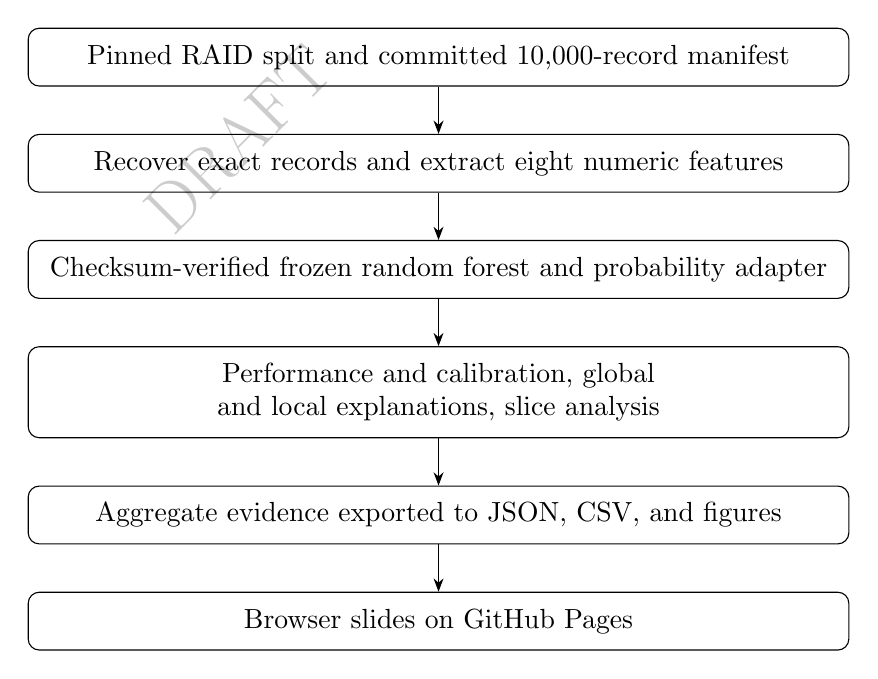
\begin{tikzpicture}[node distance=6mm, box/.style={draw, rounded corners, align=center,text width=10cm,inner sep=6pt}, flow/.style={-{Stealth}}]
\node[box] (data) {Pinned RAID split and committed 10,000-record manifest};
\node[box,below=of data] (features) {Recover exact records and extract eight numeric features};
\node[box,below=of features] (model) {Checksum-verified frozen random forest and probability adapter};
\node[box,below=of model] (audit) {Performance and calibration, global and local explanations, slice analysis};
\node[box,below=of audit] (export) {Aggregate evidence exported to JSON, CSV, and figures};
\node[box,below=of export] (pages) {Browser slides on GitHub Pages};
\draw[flow] (data)--(features); \draw[flow] (features)--(model); \draw[flow] (model)--(audit);
\draw[flow] (audit)--(export); \draw[flow] (export)--(pages);
\end{tikzpicture}
\caption{End-to-end experiment and publishing architecture}
\end{figure}
The dataset loader resolves the sample, the feature module constructs the ordered vector, the model loader verifies artifact integrity, and the audit scripts export results. The site renders those exports.
Record IDs select texts from RAID. Feature vectors feed the probability adapter, and prediction and attribution aggregates flow to the static deck.
\section{Data Sources and Contracts}
RAID records preserve domain, generator, attack, decoding, and repetition metadata for slice analysis.
The ordered features are character count, word count, average word length, punctuation count, sentence count, average sentence length, uppercase word count, and title-case word count. The model has 100 trees. The probability adapter forwards numeric feature vectors to the frozen classifier. Class 0 is Human and class 1 is AI.

Feature order is part of the contract because several columns have similar numeric ranges. Passing word counts into a sentence-count column can yield plausible output despite a malformed input. The compatibility checks verify numeric input shape, class order, and probability parity across the adapter before the model is evaluated.
The stages exchange manifest IDs, ordered feature matrices, and static JSON or CSV files.
\section{Validation and audit evidence}
Checks enforce artifact integrity, sample size, confusion-matrix parity, and consistent threshold totals.
An audit finding records a case identifier, actual class, predicted class, score, and attribution evidence.
\section{Risk Scoring, Storage and Reporting}
The classifier score estimates the AI class. The threshold control reports the resulting false positives and false negatives.

The audit precomputes a confusion matrix for each threshold from 0.00 to 1.00 in increments of 0.01. Scores exactly equal to the threshold are classified as Human. This tie rule reproduces the original decision at 0.50 and matters because a finite forest can assign the same score to many records.
Aggregate JSON, plots, and case CSV files are versioned in Git.
The analysis runs as deterministic scripts. The browser displays their saved outputs.
\section{Deployment and Operations}
The sample recovery matches published IDs against the pinned dataset. The audit export checks the confusion matrix against the original evaluation. The local environment and recovered text are excluded from Git. The deployed deck loads precomputed evidence.
Pinned revisions and explicit validation checks preserve reproducibility. The UI presents an unavailable-data message when an audit asset fails to load.
\chapter{Results and Discussion}
Artifact checks cover the sample count, bins, error totals and slices. Edge tests exercise slide navigation and the analysis controls.
\section{Measured functional run}
\begin{table}[htbp]\centering
\caption{Frozen-model results on the exact RAID sample}
\begin{tabular}{lr}\toprule Measure & Value \\ \midrule
Accuracy & 60.99\% \\
AI precision & 59.66\% \\
AI recall & 67.90\% \\
ROC-AUC & 0.645 \\
Brier score & 0.2890 \\
Ten-bin expected calibration error & 21.02\% \\
False positives & 2,296 \\
False negatives & 1,605 \\ \bottomrule
\end{tabular}\end{table}
\auditfigure{0.67}{confusion_matrix.png}{Confusion matrix. Rows are actual classes and columns are predictions.}
Character and word count have a Pearson correlation of 0.91. Word and sentence count have a correlation of 0.84. These relationships can complicate interpretation when one feature changes independently. Morris ranks average word length highest. PDP shows the average response rather than the response of any one record.
\auditfigure{0.87}{feature_correlation.png}{Pearson coefficients from the 500 rows used for PDP.}
\auditfigure{0.82}{morris_sensitivity.png}{Measured Morris sensitivity.}
\auditfigure{0.95}{partial_dependence.png}{Partial dependence across the numeric inputs.}
\section{Observed outcomes}
Each of the four cases represents one cell of the confusion matrix. Five seeded reruns yielded Stable Kernel SHAP attributions across all four cases and Mixed LIME attributions for two cases. The model probabilities stayed constant. Attribution variability therefore arises even when the prediction is fixed.

The stability badges summarize three pairwise statistics over the five runs. Spearman correlation measures consistency of the absolute feature ranking. Sign agreement measures whether each feature continues to move the explained output in the same direction. Top-three overlap measures agreement on the leading features. These summaries let readers compare stable predictions with explanations that are sensitive to a method's sampling procedure.

The false-positive records averaged 1,737 characters, and the false negatives averaged 1,493. The corresponding median lengths were 1,393 and 1,405 characters, showing how the distribution tails affect the averages. Among false negatives, poetry contributed 399 records, books 276, and Reddit 227. These are counts within the error group. Comparing error rates across domains also requires the number of evaluated records in each domain.

The slice explorer compares mean absolute Kernel SHAP values with a common reference background and up to 24 explained records per group. It reports group sizes and allows comparisons by domain, generator, attack status, decoding, repetition penalty, and true class. These summaries describe the sampled groups and support hypothesis generation. They cannot isolate the effect of a single metadata field.
\section{Limitations}
The benchmark uses balanced classes and the slice attributions use a limited sample per group. Calibration and error rates depend on the evaluation population.
\section{Discussion}
\auditfigure{1.0}{calibration.png}{Reliability by score bin and score distributions by actual class.}
At the evaluated decision rule, AI scores strictly greater than 0.50 are flagged. Moving the threshold changes both kinds of error. The Brier score measures mean squared probability error, while expected calibration error summarizes the sample-weighted gap between mean scores and observed rates across bins.
\chapter{Conclusion}
The project reproduced the frozen classifier's behavior on the exact 10,000-record RAID cohort. At the original threshold, 2,704 human records and 3,395 AI records were classified correctly. The remaining 2,296 false positives and 1,605 false negatives account for 39.01\% of the cohort. In this balanced evaluation, nearly half of the human examples were flagged. That error burden makes the classifier unsuitable as the sole basis for an authorship decision under comparable conditions.

The experiments explain several aspects of this outcome. The correlation analysis shows that document-length measures move together, which complicates the interpretation of single-feature changes. Morris screening identifies average word length as the most sensitive input in the recorded analysis. Partial dependence describes how the mean model response changes across its feature settings. The what-if cases show how the same type of numerical change can affect individual records. These results describe the forest's response to stylometry and do not establish a causal relationship between writing style and authorship.

Local explanations add case-level detail. Across five seeded runs, the Kernel SHAP rankings were classified as stable for all four cases, while LIME returned mixed results for two. The underlying model probabilities were unchanged across these reruns. Thus a steady model decision can coexist with disagreement about which inputs explain it. A reviewer should consider the two explanations, their stability scores, and the input context together before interpreting an individual attribution.

Calibration provides a separate check on score interpretation. The Brier score of 0.2890 and the ten-bin calibration error of 21.02\% show substantial discrepancy between the assigned scores and outcomes on this cohort. The reliability figure and threshold sweep make that discrepancy and its practical trade-offs inspectable. The central deliverable is a reproducible record of model behavior, from the pinned sample and frozen artifact through the published charts and interactive cases.

\chapter{Future Enhancements}
\section{Validate transfer and report uncertainty}
Evaluate the unchanged classifier on an independently sampled cohort containing unseen generators and domains. Preserve source groups when partitioning examples so near-duplicate material does not appear on both sides of a comparison. Report the observed class prevalence, sample sizes, and confidence intervals for each group. A grouped bootstrap would help distinguish genuine shifts in error from variability caused by small samples or closely related documents. The current balanced cohort can remain a fixed regression check for the evaluation pipeline.

\section{Strengthen calibration and threshold evaluation}
Reserve separate data for calibrator fitting and final evaluation. Compare the original scores with calibration methods such as isotonic regression or sigmoid calibration, then report reliability curves and Brier scores on held-out data. Evaluate threshold choices against an explicit cost model for false flags and misses. Reporting thresholds together with class prevalence and uncertainty would make the results more informative for a particular review setting.

\section{Test explanation robustness}
Vary the reference background, random seed, and sample budget independently to quantify their effects on attribution rankings. Extend the stability study beyond four selected cases with a stratified sample of correct predictions and both error types. Where features are closely related, add grouped perturbation experiments and compare their conclusions with the recorded single-feature results. Report uncertainty intervals for group-level attribution summaries and record which comparisons are consistently supported across runs.

\chapter*{Appendix: Reproduction and Reporting Evidence}
\addcontentsline{toc}{chapter}{Appendix: Reproduction and Reporting Evidence}
The \href{https://aditya-ranjan1234.github.io/Interpretml-AI-Text-Detector/}{GitHub Pages deck} is the published reporting surface. The project repository contains the manifest, model checksum, audit exports, chart sources, and browser verification script.
\begin{thebibliography}{99}
\bibitem{paper1} Dutta Chowdhury, S. A., España-Bonet, C., \& Van Genabith, J. (2026). Formatting and Surface Feature Confounds in AI Text Detection: A Clever Hans Effect. \emph{Findings of EMNLP 2026, 22266–22277}. \href{https://aclanthology.org/2026.findings-emnlp.1051/}{Publication record}.
\bibitem{paper2} El Attar, A., Dönmez, Ç., Maurer, M., \& Falenska, A. (2026). A Systematic Analysis of Linguistic Features in AI-Generated English Text Detection Across Domains and Models. \emph{Findings of IJCNLP-AACL 2026, 181–208}. \href{https://aclanthology.org/2026.findings-aacl.10/}{Publication record}.
\bibitem{paper3} Xia, M., Stańczak, K., \& Roth, B. (2026). Explaining Generalization of AI-Generated Text Detectors Through Linguistic Analysis. \emph{EACL 2026, 6524–6546}. \href{https://aclanthology.org/2026.eacl-long.307/}{Publication record}.
\bibitem{paper4} Shan, Z., Lee, Y., \& Hao, S. (2026). AI Writers Have a Consistent Stylometric Footprint, but AI Editors Do Not. \emph{EMNLP}. \href{https://aclanthology.org/2026.emnlp-main.1725/}{Publication record}.
\bibitem{paper5} Tufts, B., Zhao, A., \& Li, S. (2025). A Practical Examination of AI-Generated Text Detectors for Large Language Models. \emph{Findings of NAACL 2025, 4839–4856}. \href{https://aclanthology.org/2025.findings-naacl.271/}{Publication record}.
\bibitem{paper6} Doughman, J. et al. (2025). Exploring the Limitations of Detecting Machine-Generated Text. \emph{COLING 2025, 4274–4281}. \href{https://aclanthology.org/2025.coling-main.288/}{Publication record}.
\bibitem{paper7} Yang, X. et al. (2024). DNA-GPT: Divergent N-Gram Analysis for Training-Free Detection of GPT-Generated Text. \emph{ICLR 2024}. \href{https://arxiv.org/abs/2305.17359}{Publication record}.
\bibitem{m4} Wang, Y. et al. (2024). M4: Multi-generator, Multi-domain, and Multi-lingual Black-Box Machine-Generated Text Detection. \emph{EACL 2024, 1369–1407}. \href{https://aclanthology.org/2024.eacl-long.83/}{Publication record}.
\bibitem{paper8} Li, Y. et al. (2024). MAGE: Machine-generated Text Detection in the Wild. \emph{ACL 2024, 36–53}. \href{https://aclanthology.org/2024.acl-long.3/}{Publication record}.
\bibitem{paper9} Bao, G. et al. (2024). Fast-DetectGPT: Efficient Zero-Shot Detection of Machine-Generated Text via Conditional Probability Curvature. \emph{ICLR 2024}. \href{https://arxiv.org/abs/2310.05130}{Publication record}.
\bibitem{paper10} Verma, V., Fleisig, E., Tomlin, N., \& Klein, D. (2024). Ghostbuster: Detecting Text Ghostwritten by Large Language Models. \emph{NAACL-HLT 2024, 1702–1717}. \href{https://aclanthology.org/2024.naacl-long.95/}{Publication record}.
\bibitem{paper11} Hans, A. et al. (2024). Spotting LLMs With Binoculars: Zero-Shot Detection of Machine-Generated Text. \emph{ICML 2024, PMLR 235, 17519–17537}. \href{https://proceedings.mlr.press/v235/hans24a.html}{Publication record}.
\bibitem{raid} Dugan, L. et al. (2024). RAID: A Shared Benchmark for Robust Evaluation of Machine-Generated Text Detectors. \emph{ACL 2024, 12463–12492}. \href{https://aclanthology.org/2024.acl-long.674/}{Publication record}.
\bibitem{paper12} Wang, Y. et al. (2024). Stumbling Blocks: Stress Testing the Robustness of Machine-Generated Text Detectors Under Attacks. \emph{ACL 2024, 2894–2925}. \href{https://aclanthology.org/2024.acl-long.160/}{Publication record}.
\bibitem{paper13} Krishna, S. et al. (2024). The Disagreement Problem in Explainable Machine Learning: A Practitioner's Perspective. \emph{Transactions on Machine Learning Research}. \href{https://arxiv.org/abs/2202.01602}{Publication record}.
\bibitem{paper14} Laberge, G., Pequignot, Y. B., Marchand, M., \& Khomh, F. (2024). Tackling the XAI Disagreement Problem with Regional Explanations. \emph{AISTATS}. \href{https://proceedings.mlr.press/v238/laberge24a.html}{Publication record}.
\bibitem{paper15} Hill, D., Masoomi, A., Torop, M., Ghimire, S., \& Dy, J. (2024). Boundary-Aware Uncertainty for Feature Attribution Explainers. \emph{AISTATS}. \href{https://proceedings.mlr.press/v238/hill24a.html}{Publication record}.
\bibitem{paper16} Liang, W., Yuksekgonul, M., Mao, Y., Wu, E., \& Zou, J. (2023). GPT detectors are biased against non-native English writers. \emph{Patterns, 4(7), 100779}. \href{https://doi.org/10.1016/j.patter.2023.100779}{Publication record}.
\bibitem{paper17} Mitchell, E., Lee, Y., Khazatsky, A., Manning, C. D., \& Finn, C. (2023). DetectGPT: Zero-Shot Machine-Generated Text Detection using Probability Curvature. \emph{ICML 2023, PMLR 202, 24950–24962}. \href{https://proceedings.mlr.press/v202/mitchell23a.html}{Publication record}.
\bibitem{paper18} Macko, D. et al. (2023). MULTITuDE: Large-Scale Multilingual Machine-Generated Text Detection Benchmark. \emph{EMNLP 2023, 9960–9987}. \href{https://aclanthology.org/2023.emnlp-main.616/}{Publication record}.
\bibitem{paper19} Rodriguez, J. D., Hay, J., Gros, D., Shamsi, J. A., \& Srinivasan, P. (2022). Cross-Domain Detection of GPT-2-Generated Technical Text. \emph{NAACL-HLT 2022, 1213–1233}. \href{https://aclanthology.org/2022.naacl-main.88/}{Publication record}.
\bibitem{paper20} Chouraqui, G., Cohen, L., Einziger, G., \& Leman, L. (2022). A geometric method for improved uncertainty estimation in real-time. \emph{UAI}. \href{https://proceedings.mlr.press/v180/chouraqui22a.html}{Publication record}.
\bibitem{paper21} Uchendu, A., Ma, Z., Le, T., Zhang, R., \& Lee, D. (2021). TURINGBENCH: A Benchmark Environment for Turing Test in the Age of Neural Text Generation. \emph{Findings of EMNLP 2021, 2001–2016}. \href{https://aclanthology.org/2021.findings-emnlp.172/}{Publication record}.
\bibitem{kernel} Covert, I., \& Lee, S.-I. (2021). Improving KernelSHAP: Practical Shapley Value Estimation Using Linear Regression. \emph{AISTATS}. \href{https://proceedings.mlr.press/v130/covert21a.html}{Publication record}.
\bibitem{paper22} Gupta, C., \& Ramdas, A. (2021). Distribution-Free Calibration Guarantees for Histogram Binning without Sample Splitting. \emph{ICML}. \href{https://proceedings.mlr.press/v139/gupta21b.html}{Publication record}.
\bibitem{lime} M. T. Ribeiro, S. Singh, and C. Guestrin (2016). Why Should I Trust You? Explaining the Predictions of Any Classifier. \emph{KDD}. \href{https://doi.org/10.1145/2939672.2939778}{Publication record}.
\bibitem{shap} S. M. Lundberg and S.-I. Lee (2017). A Unified Approach to Interpreting Model Predictions. \emph{NeurIPS}. \href{https://arxiv.org/abs/1705.07874}{Publication record}.
\end{thebibliography}

\end{document}
